\begin{center}
    \begin{figure}[H]
        \centering

        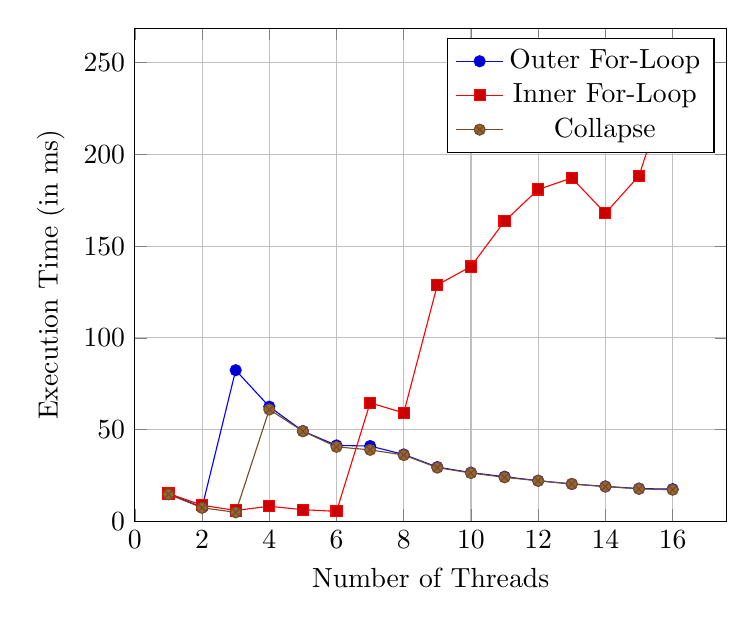
\begin{tikzpicture}
            \begin{axis}[
                title={},
                width=0.75\textwidth,
                xlabel={Number of Threads},
                ylabel={Execution Time (in ms)},
                xmin=0,
                ymin=0,
                grid=major
            ]
                \addplot coordinates {
                    (1,15.3049)(2,7.56055)(3,82.3768)(4,62.4837)(5,49.1818)(6,41.3728)(7,41.0167)(8,36.4371)(9,29.5454)(10,26.5446)(11,24.3035)(12,22.1388)(13,20.3482)(14,19.0172)(15,17.8612)(16,17.5258)
                };
                \addlegendentry{Outer For-Loop}

                \addplot coordinates {
                    (1,15.1618)(2,8.75195)(3,5.91315)(4,8.1956)(5,6.32605)(6,5.4254)(7,64.5677)(8,59.0846)(9,128.857)(10,138.879)(11,163.544)(12,180.893)(13,187.137)(14,167.894)(15,188.379)(16,244.342)
                };
                \addlegendentry{Inner For-Loop}       

                \addplot coordinates {
                    (1,14.7323)(2,7.3617)(3,4.90575)(4,60.9359)(5,49.1117)(6,40.5794)(7,38.9427)(8,36.1211)(9,29.2632)(10,26.3274)(11,23.971)(12,22.0927)(13,20.3762)(14,18.9155)(15,17.6862)(16,17.22)
                };
                \addlegendentry{Collapse}
            \end{axis}
        \end{tikzpicture}
        \caption{Grayscale Performance Tests dice.png}
    \end{figure}
\end{center}